\documentclass[twoside,11pt,ShortChapTitles]{BYUTextbook}

\usepackage{soul}
\renewcommand{\vec}[1]{\ensuremath{\mathbf{#1}}}
\usepackage{siunitx}
\sisetup{round-mode = figures,
  round-precision = 3, scientific-notation=true}
  \usepackage{marginfix}

\usepackage{mathtools}
\renewcommand{\chaptername}{Lab}

\setcounter{chapter}{9}

\begin{document}
\chapter[Numerical Modeling III]{Numerical Modeling and Uncertainty}
\section{Assignment: Modeling and Uncertainty}

In this lab we will finally test our numerical modeling of a projectile. We
will use our spring cannons and shoot balls that have large drag
coefficients. \textbf{Be careful not to shoot people, including you--don't
look down the barrel of the cannon! Also, don't load the cannon by pushing
down on the ball in the cannon, set the spring first and then gently put in
the ball If you push on the Styrofoam balls you will have flat balls that
don't match our models. }

There is too much to do in this lab to have everyone do all the parts. You
will have to split up your group. So how do you record all the experiment if
you only do part of it? The way this is done is to write down the results
obtained by the other subgroups, and refer to their lab notebooks for the
details.

To help determine how you will break things up, there are four major parts to this lab:

\begin{enumerate}
\item Predicting the range of the ball using Euler's method plus Monte Carlo error propagation.
\item Measuring the drag coefficient of the Styrofoam ball
\item Measuring the initial velocity of the Styrofoam ball
\item Actually firing the cannon and confirming your measurements

\end{enumerate}
\subsection{Predicting the range of the ball}
\begin{enumerate}
\item \textbf{Predict} the maximum range for the path of a Styrofoam ball
(or a plastic ball if we don't have any Styrofoam balls) shot out of the
spring cannon. Do this with a numerical model of the ball's flight path
written by one (or more) of the members of your group that has been changed
so that it can find the error estimate as described in today's lab reading.

\item Determine the uncertainty in your prediction with your new code that
chooses values for the input parameters randomly\sidenote{Make use of the normal function from numpy as described in the chapter introduction.} from within the parameter
uncertainty ranges. This is actually more efficient than trying to pick
values in a non-random way to cover all possible combinations of
uncertainties! You will need to take about $100$ or more sets of parameters
to get a good estimate, but if you built your code so you can easily change
your parameters, this will go quickly (if you put actual numbers into your
equations in the previous labs, it might be faster to fix your Python code
first to make this part go more quickly. If you need help, call me over).




\item You want to do this for every variable that has
uncertainty, and you want to do the calculation many times so you get a good
idea of the precision of your answer. Here is a figure showing an example
result:

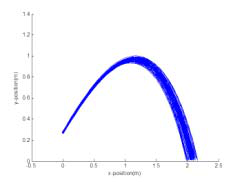
\includegraphics[scale=0.6]{Lab9_figs/old_images-058.png}

\item Additionally, you need to be able to find where the ball hits the ground.  You can do this by either changing your Euler \code{for} loop into a \code{while} loop, or by inserting an \code{if}\sidenote{The command \code{break} will tell your program to exit whatever loop it is currently in.} statement.

\end{enumerate}
\subsection{Finding the drag coefficient}
\begin{enumerate}
\item You will need to find the drag coefficient. A subteam should find a
value (and uncertainty) for the drag coefficient. One way to do this is to
use our high speed cameras and film the ball dropping. Since there is
significant air resistance, the ball will reach terminal speed. At this
point, there is no acceleration, so
\begin{eqnarray*}
\sum F &=&0=R-F_{g} \\
F_{g} &=&R \\
mg &=&\frac{1}{2}D\rho Av^{2}
\end{eqnarray*}%
so%
\[
D=\frac{2mg}{\rho Av^{2}}
\]%
Since we know or can measure everything except $D,$ we can solve for $D.$
Use $g=\left( 9.8004\pm 0.0001\right) \text{m}/\text{s}$ and $\rho =\left(
1.23\pm 0.1\right) \text{kg}/\text{m}^{3}.$

\begin{itemize}
\item The rest of the values you will need to measure. Use the digital
camera and Logger Pro to estimate the terminal velocity. You will have to
drop the ball from high up to get a good value (you have to give it time to
reach terminal velocity). Near the ground there can be problems due to the
air flow hitting the ground, so don't use positions that are close to the
ground.

\item I suggest you have a team of people from your group do this while a
second team modify your Python code. Remember you need an uncertainty in $D.$
\end{itemize}
\end{enumerate}
\subsection{Finding the launch speed of the styrofoam ball}
\begin{enumerate}
\item You will need to find the launch speed of the ball, with its uncertainty. Air resistance makes a big enough impact that using Logger Pro and Video Analysis isn't feasible. Instead, you can find the velocity using a photogate set up where the ball exits the cannon. A few notes:
\begin{itemize}
\item As a reminder, a photogate shows the time that a laser was blocked, so to turn that into a speed, you'll need to divide a distance by the time

\item You can get uncertainty in time through making several measurements, then finding the average and standard deviation of the mean.

\item The distance to use is a little more complicated than just the uncertainty in the diameter of the ball. If the laser isn't perfectly aligned with the center of the ball as it goes through, then the length of the ball that blocks the laser will be shorter than the diameter (i.e. less ball will travel through the laser beam). With a bit of geometry, you can show that \[d_{beam} = d_{ball}\sqrt{1-\alpha^2}\] where $d_{beam}$ is the amount of ball that went through the beam, $d_{ball}$ is the actual diameter of the ball, and $\alpha$ is how far from the center (as a ratio of the radius) of the ball the beam is.

Here's an example on how to use this equation: imagine I have a ball with a diameter of 2cm, and I think that I can confidently keep the laser within 0.5 cm of the center of the ball (50\% of the radius), the smallest diameter that I would expect to pass through the beam would be: 
\[d_{beam} = 2cm * \sqrt{1-0.5^2} = 1.73  cm \approx 1.7 cm \]
Since I'd expect my diameter  to be somewhere between that number and 2 cm, I'd quote the diameter that passes through the beam to be $ 1.85 \pm 0.15$ cm.
\end{itemize}
\end{enumerate}

\subsection{Actually Firing the cannon}
\begin{enumerate}
\item Verify the prediction. Did the ball land within your error range? If
you use the digital cameras again for this part, you can determine if the
flight path falls within the range of possible flight paths. A figure like
the following might help you decide:

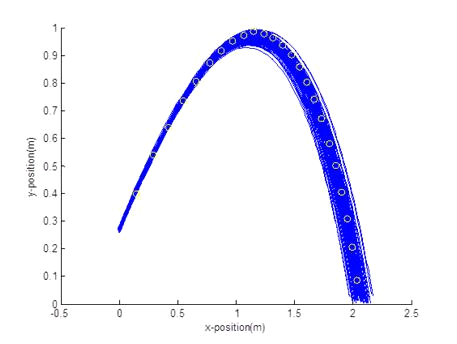
\includegraphics[scale=0.5]{Lab9_figs/old_images-059.png}

\item Does the data support your modeling prediction? If not, what is likely
the problem?

\begin{itemize}
\item In your discussion make sure your other team members understand the
part of the project that you did.

\item You might consider having a third team collect data for the ball shot
with the digital camera while the first two teams are working on the drag
coefficient and the numerical prediction.
\end{itemize}


\end{enumerate}

\end{document}
